\documentclass[12pt]{article}
\usepackage[margin=1in]{geometry}
\usepackage{amsmath}
\usepackage{graphicx}

\title{E155 Final Project Status Report: $\mu$Mudd Mark V Debugging and Lab 6 Revision}
\author{Christopher Ferrarin and Kaveh Pezeshki}
\date{28 November 2018}

\begin{document}
	\begin{LARGE}
	\noindent
		E155 
		Final 
		Project 
		Status
		Report: 
		$\mu$Mudd 
		Mark V \\
		Debugging 
		and 
		Lab 
		6 
		Revision
	\end{LARGE}

	\vspace{0.2cm}
	
	\begin{large}
	Christopher Ferrarin and Kaveh Pezeshki
	
	28 November 2018
	\end{large}

\section{Completed Deliverables Status}
Below is a summary of project deliverables and deliverable status:

	\begin{center}
	\begin{tabular}{p{6cm}p{5cm}p{4cm}}
	Deliverable Category & Deliverable Name & Deliverable Status\\
	\hline
	Identifying blocking $\mu$Mudd Bugs & Identifying MCU programming failure & Complete \\
	Revising $\mu$Mudd to allow MCU functionality & Hardware modification of pre-existing PCBs & Complete \\
	& New JTAG cable & Complete \\
	& Modified schematic and layout & In progress \\
	& Completed  $\mu$Mudd respin & Not started \\
	Reworking Lab 6 & Rewrite EasyPIO.h with SAM4S support & Complete \\
	& Integrate MCP3002, photodiode, and BlueSMiRF & Complete \\
	& Formally write up lab for student readability & Not started \\
	Testing other labs & Lab 4 & Not started \\
	& Lab 5 & Not started \\
	& Lab 7 & Not started
	\end{tabular}
	\end{center}

\section{Deliverable Status: Revised $\mu$Mudd}

A major component of this final project is identifying errors in the PCB design that lead to a non-programmable MCU. We have identified two errors which when solved allowed MCU programming

\subsection{Schematic Errors}

\subsubsection{MCU ERASE Pin}
The largest problem with the current $\mu$Mudd design lies in the MCU ERASE pin, which reinitializes the onboard flash and resets the processor. The ERASE pin can also serve as general-purpose I/O after configuration. \footnote{SAM4S Series Datasheet p37}

On boot, ERASE must be held low to prevent flash erase and reinitialization of the processor. On the current $\mu$Mudd, ERASE was tied to a general I/O pin on the Cyclone IV FPGA. The connection can be seen in the following schematic:

\begin{center}
	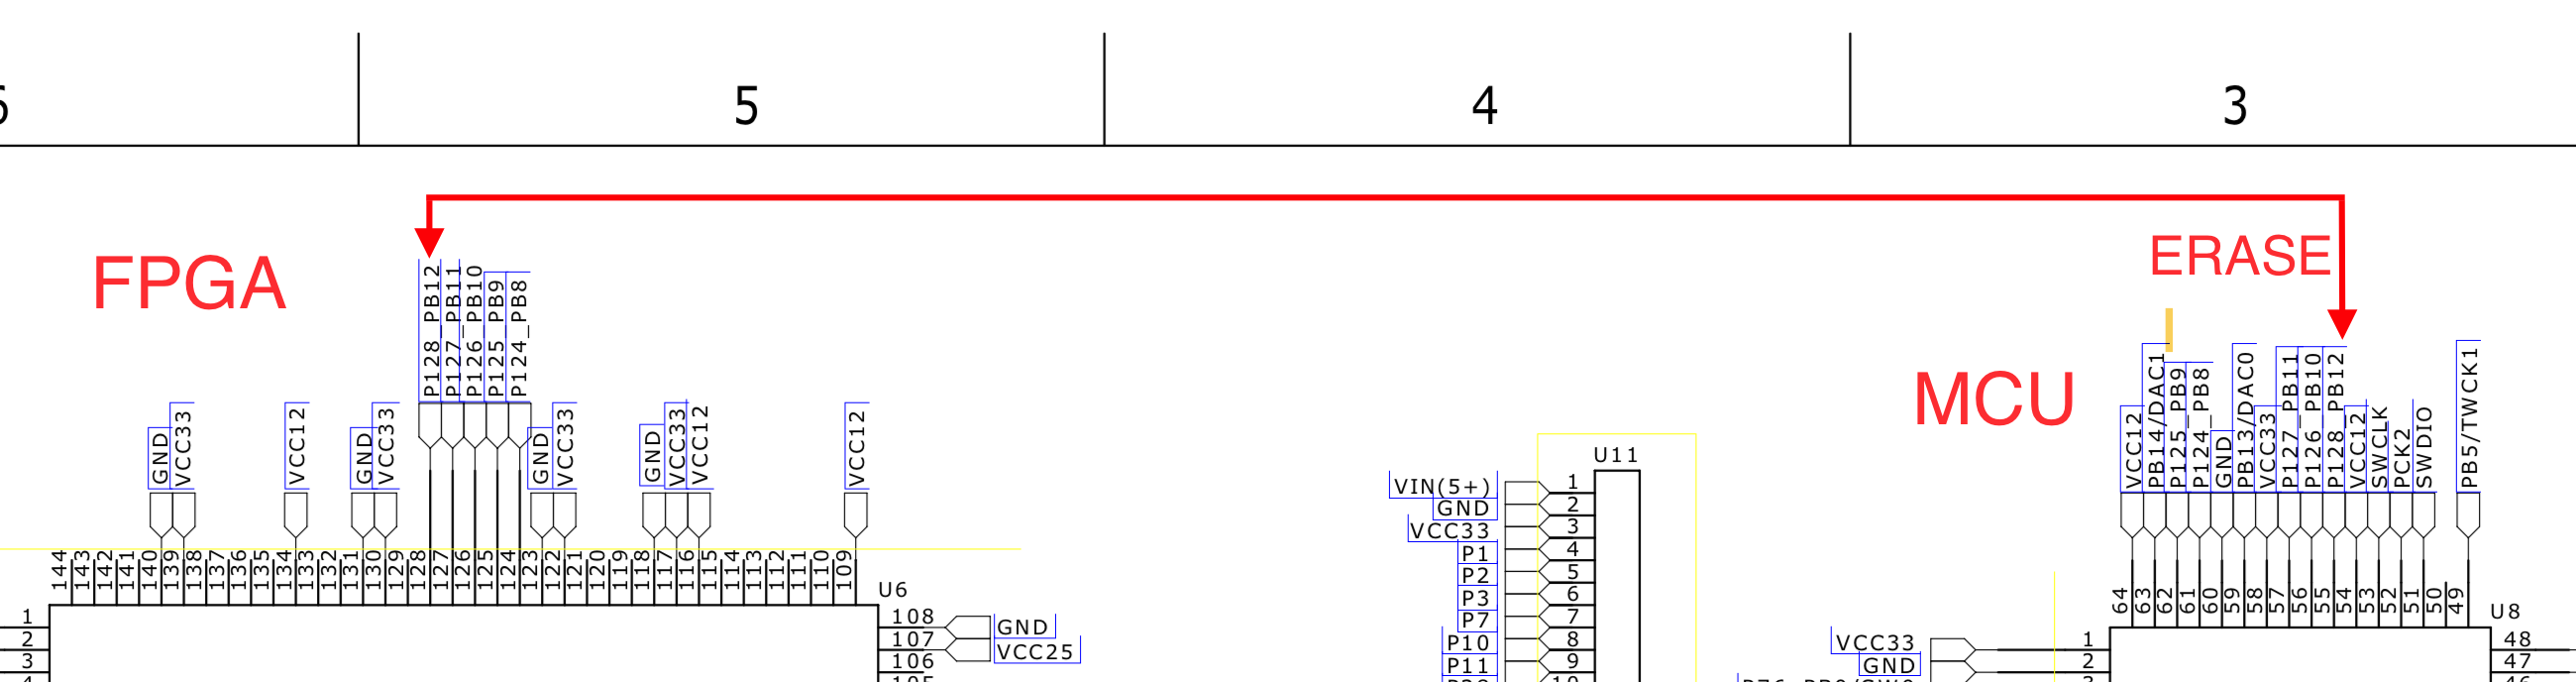
\includegraphics[width=16cm]{erase_error.png}
	\caption{The marked connection ties ERASE on the MCU to pin 128 on the FPGA}
\end{center}

The ERASE pin contains a 100k$\Omega$ pull-down resistor\footnote{SAM4S Series Datasheet p37}.An unconfigured Cyclone IV I/O pin contains a 25k$\Omega$ pull-up resistor \footnote{Cyclone IV Device Handbook p6-3}. This creates a voltage divider circuit as shown below:

\begin{center}
	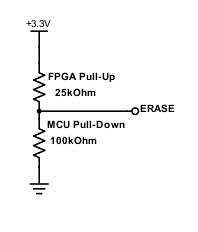
\includegraphics[width=6cm]{resistor_divider.png}
\end{center}

This provides a predicted voltage of 2.64V on the MCU ERASE pin, close to the 2.86V we observed. This is a high logic level which prevented FPGA programming.

\subsubsection{MCU Power Supply}

The MCU requires a 3.3V and 1.2V power supply. It can be powered via one 3.3V supply, and use an internal regulator to generate 1.2V, or it can be powered with an external 3.3V and a 1.2V supply. The dual-regulator design of the current board can introduce startup issues if timing is not correct.

\begin{figure*}
	\begin{center}
	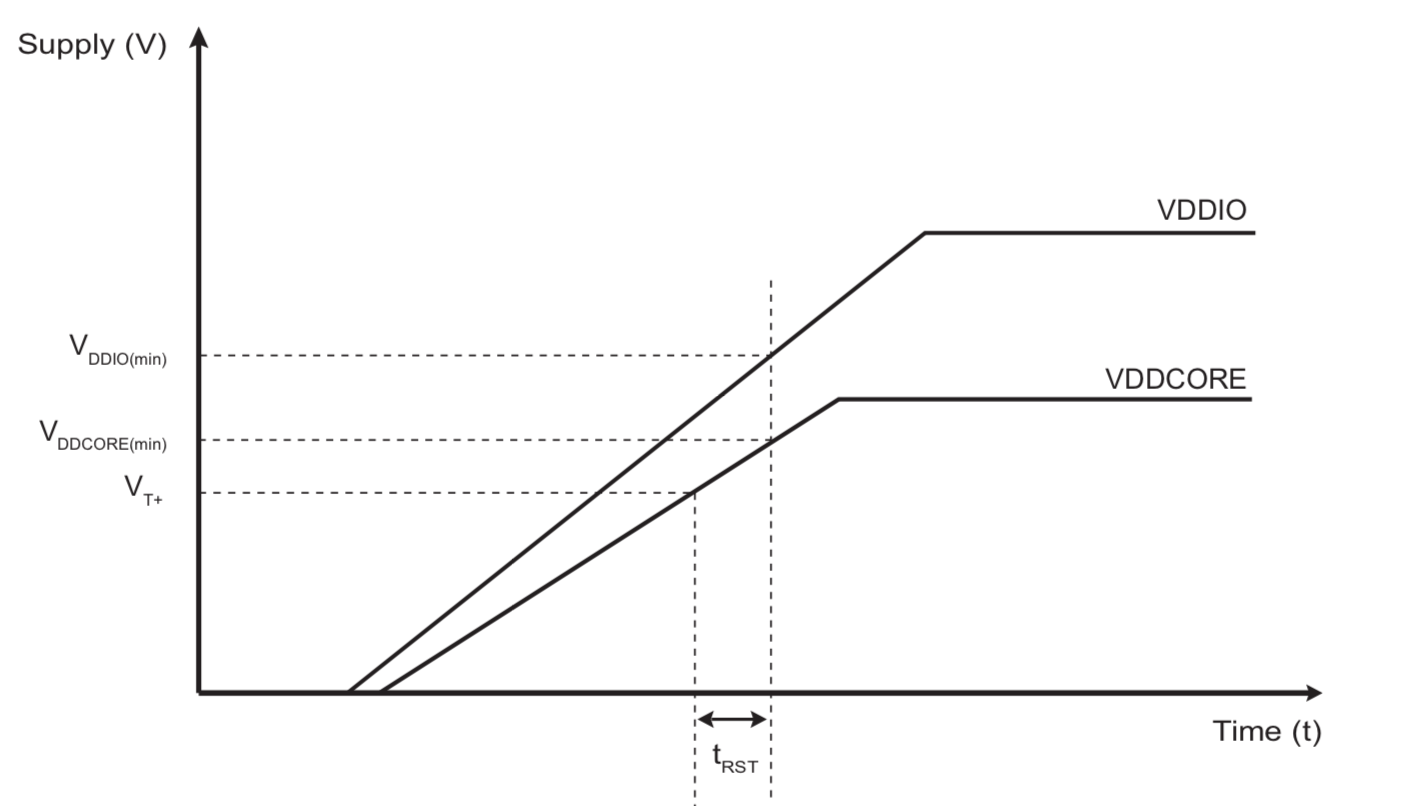
\includegraphics[width=13cm]{power_timing.png}
	\caption{Timing requirements for the 1.2V (VDDCORE) and 3.3V (VDDIO) supplies, taken from the SAM4S Series Datasheet p27}	
	\end{center}
\end{figure*}

We believe that these potential timing errors can cause system instability, as we observed an unresponsive MCU after startup that could only be solved with a full erase and reset.

\subsubsection{JTAG connector pinout}

The MCU JTAG connector was incorrectly wired on the current $\mu$Mudd. This led to wiring errors in the I$^2$C connection

\subsection{Schematic and Layout Changes}

We have implemented a set of changes to the schematic to solve the problems noted above and to improve the PCB, but have not yet propagated these changes to the layout. These include:

\begin{enumerate}
	\item Moving ERASE control to the MCU RESET pushbutton. RESET will be accessible through JTAG
	\item Powering the 1.2V MCU VDDCORE with the onboard regulator, and adding necessary passives
	\item Correcting JTAG and I$^2$C wiring errors
	\item Replacing 0.1" pitch JTAG connectors with 0.05" pitch SWD connectors. This adds compatibility with J-Link EDU Mini programmers
	\item Adding 0.1'' jumpers on critical MCU pin connections to assist debugging 
\end{enumerate}

\newpage
\section{Deliverable Status: Reworking Lab 6 and EasyPIO.h}

\subsection{Reworking Lab 6}
The proposed Lab 6 architecture is shown in detail below:

\begin{center}
	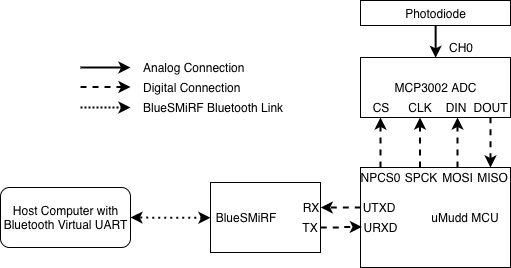
\includegraphics[width=14cm]{blockdiagram.png}
\end{center}

To maintain a low lab cost we exchanged one BlueSMiRF and the serial display for a computer with an integrated Bluetooth module. We added a MCP3002 ADC to retain the datasheet interpretation component of the lab.

We have successfully demonstrated Bluetooth communication between two computers, using a Bus Pirate as a USB to UART converter. We have also successfully demonstrated voltage measurement with the MCP3002 through a SAM3S/SAM4S SPI peripheral.

In reworking Lab 6, we still need to write an updated version of the lab manual and polish it so that it easily readable by a future student. We also seek to implement any recommendations we receive in our presentation for ways to improve this lab, as the replacement of the web server with a Bluetooth link may render the lab simpler than we'd like.

\subsection{Targeting easyPIO.h for the SAM4S}

We have created an I/O header file, easySamIO.h, which provides Arduino-style access to the GPIO, timer, UART, and SPI peripherals on the SAM4S. In the style of easyPIO.h, we provide only the configuration and functionality necessary to complete labs. We aim to provide adequate inline documentation for students to add functionality as necessary. This documentation includes functional descriptions of memory access, references to the datasheet, and brief descriptions of other peripheral features.

In total, we have completed implementation of the PIO, timer, SPI, and UART peripherals, but still need to provide access to additional ports of the PIO peripheral, additional channels of the timer peripheral, and additional clock routing for the FPGA on the $\mu$Mudd.

We believe a thorough and well-documented EasySamIO.h will be more useful for lab 4,5, and 7 bringup than testing labs 4,5, and 7 as discussed in the lab manual.

\clearpage
\section{Appendix 1: Updated Schematic}
\clearpage
\section{Appendix 2: C Code}
\subsection{EasySamIO.h}
\pagebreak
\subsection{lab6.c}
\end{document}
